\documentclass[a4paper,10pt]{article}
\renewcommand{\baselinestretch}{1.05}

\usepackage{times}
\usepackage{lipsum}
\usepackage[T1]{fontenc}
\usepackage[utf8]{inputenc}
%\usepackage[xetex]{graphicx} % when you compile with xelatex
\usepackage[pdftex]{graphicx} % when you compile with pdflatex
\usepackage{tikz}
\usepackage{epstopdf}
\usepackage{float}
\usepackage{mathtools}
\usepackage{url}
\usepackage[english]{babel}
\usepackage{paralist}
\usepackage{enumitem}
\usepackage{multicol}
\usepackage{pdfpages}
\usepackage{placeins}
\usepackage{titlesec}
\usepackage{verbatim}
\usepackage{xcolor}
\usepackage[ampersand]{easylist}
\usepackage{listings}
\usepackage{tabularx,rotating}
\usepackage{lscape}
\usepackage{booktabs}
\usepackage{afterpage}
\usepackage{capt-of}
\usepackage{adjustbox}
\definecolor{light-gray}{gray}{0.97} %the shade of grey that stack exchange uses

\definecolor{codegray}{rgb}{0.5,0.5,0.5}
\lstdefinestyle{mystyle}{
    language = Java,
    numberstyle=\tiny\color{codegray},
    basicstyle=\ttfamily\footnotesize,
    breakatwhitespace=false,         
    breaklines=true,                 
    captionpos=b,                    
    keepspaces=true,                 
    numbers=left,   
    numbersep=5pt,                  
    showspaces=false,                
    showstringspaces=false,
    showtabs=false,                  
    tabsize=2
    % frame=tb
}

\lstset{style=mystyle}

\titlespacing*{\section}{0pt}{1\baselineskip}{0.1pt}
\titlespacing*{\subsection}{0pt}{1\baselineskip}{0.1pt}
\titlespacing*{\chapter}{10pt}{1\baselineskip}{0.1pt}


\usepackage{geometry}
 \geometry{
 a4paper,
 total={170mm,257mm},
 left=20mm,
 top=20mm,
 }



\usepackage{dcolumn}
\newcolumntype{d}[2]{D{.}{.}{#1}}

%%%%%%%%%%%% layout %%%%%%%%%%%%%%%%%
%\usepackage[margin=3cm]{geometry}
% you might enhance readability by increasing the distances between lines:
%\renewcommand{\baselinestretch}{1.1}

%%%%%%%%%%% mathematics %%%%%%%%%%%%%%%%%%
\usepackage{amsmath,amsfonts,amssymb}

%%%%%%%%%%%%% theorems %%%%%%%%%%%%%%%%
\usepackage{amsthm}

\theoremstyle{plain}
\newtheorem{theorem}{th}
\newtheorem{corollary}{cor}
\newtheorem{proposition}{prop}
\newtheorem{lemma}{lem}
\newtheorem{assumption}{ass}

\theoremstyle{definition}
\newtheorem{definition}{def}
\newtheorem{example}{ex}
\newtheorem{remark}{rem}
\newtheorem{notation}{not}
\newtheorem{guess}{Hypothesis}

\newcommand\mynote[1]{\textcolor{red}{#1}}
% \renewcommand\mynote[1]{} % Uncomment this to remove notes

%%%%%%%%%%%%algorithms %%%%%%%%%%%%%%%%%%%
\usepackage{boxedminipage}
\usepackage{algpseudocode}
\usepackage{hyperref}

%%%%%%%%% bibliography style %%%%%%%%%%%%%
\usepackage{natbib}

\title{\rule{\textwidth}{0.8pt} \vspace*{0.2cm} \\ {\Huge \bf AutoComment } \\ Comment Generation in Java Code}
\author{    Navin Raj Prabhu \\ 
            TU Delft \\
            \and
            Jonathan Katzy \\
            TU Delft \\
            \and
            Rafail Skoulos \\
            TU Delft \\
            \and
            Thomas Pfann \\
            TU Delft 
}
\date{October, 2019 \\ \vspace*{0.5cm}
            \rule{\textwidth}{0.8pt}}

%%%%%%%%%%%%%%%% start document %%%%%%%%%%%
\begin{document}

%%%%%%%%%%%%%%% front page %%%%%%%%%%%%%%%%

% \thispagestyle{empty}


% \vspace*{3cm}

% \noindent
\maketitle

% \begin{center}
% \rule{\textwidth}{0.8pt}
% {\Huge\bf
% \noindent
% AutoComment \\
% }
% {\Huge
% Comment Generation in Java Code
% }
% \rule{\textwidth}{0.8pt}
% \end{center}


% \vspace*{-8pt}
% \noindent
% \rule{\textwidth}{0.8pt}

% \begin{center}
% {
% }
% \end{center}
% \vspace*{1.5cm}

% \begin{center}
% {\large\bf
% Navin Raj Prabhu, Jonathan Katzy, Rafail Skoulos, and Thomas Pfann \\ 
% } 
% {\small
% TU Delft
% }

\maketitle

% \vspace*{1cm}
% \end{center}

% \newpage
%%%%%%%%%%%%%%%%%%%%%%% main contents %%%%%%%%%%%%%%%%%
% \setlength{\columnsep}{30pt}


%%%%%%%%%%%%%%%%%%%%%%%%%%%%%%%%%%%%%%%%%%%%%%%%%%%%%%%%%%%%%%%%

% \tableofcontents
% \newpage
\begin{multicols*}{2}
{\itshape
\section*{Abstract} 
Commenting large code databases is crucial for code comprehension and efficient maintenance of a code base. Therefore, automatic code generation would be incredibly beneficial for both programmer and future maintainer of the code. In this paper, we propose a comment generator model using new state of the art techniques developed in the previous years, based on code2seq\cite{alon2018code2seq} for comment generation in Java code. With the DeepCom\cite{hu2018deep} as the baseline, the paper focuses on replicating the code2seq model with added capabilities such as, predicting natural language (Method-1) and modified ASTs (Method-2). The results shows us that, Method-2, is capable of understanding the syntactic and semantic meaning of java codes to generate comments automatically, but suffers from the incapability to generate longer and complete comments, hence leading to a poor BLEU-4 score when compared to the baseline. The source code and the dataset of the project can be found in - \url{https://github.com/LRNavin/AutoComments}.
%%%%%%%%%%%%%%%%%%%%%%%%%%%%%%%%%%%%%%%%%%%%%%%%%%%%%%%%%%%%%%%%
}

\bigskip\noindent
\textbf{Keywords: comment generation, deep learning, machine learning, LSTM, Code2Seq, Software Development, Java}

\section{Introduction}
For large software systems, the maintenance phase tends to
have a comparatively longer duration than all the previous
life-cycle phases taken together \cite{aggarwal2002integrated}. A large part of the maintenance cycle is software comprehension. So much so that around 59\% of all time spent during the software development life cycle is spent on understanding of the code base. This due to time constraints and tight scheduling of projects which results into mismatching of code comments, completely omitting comments, or not updating comments of patched code in the database \cite{hu2018deep}. This has resulted in much research being conducted on automatic generation of comments given non-commented source code. Some of the first research on this subject done by Sridhara et al. \cite{sridhara2010towards} \cite{sridhara2011automatically} \cite{sridhara2011generating} focuses on automatic comment creation for certain statements and methods with their parameters respectively. 
This really brought about the use of automatic learning to aid programmers with automatic comment suggestion. 

The standard encoder decoder framework has proven to be highly effective in comment generation, as shown in \cite{alon2018code2seq}. The fully connected layer between encoder and decoder is represented by Long Short-Term Memory (LSTM) which are a form of Recurrent Neural Network (RNN). Due to LSTMs innate feedback connection, it can in addition to processing singular data points such as images, process time-series data such as speech and video. This feedback feature makes it particularly powerful within the field of automatic comment generation. Feedback allows an LSTM to cope with the lag between different important and characteristic events within code.

First we will first give an overview of the current state of the art in section \ref{background}. Then we propose a novel design for a comment generating model, explaining the architecture and specific design choices in section \ref{design}. We describe the experimental setup, results and discussion in sections \ref{setup}, \ref{results}, and \ref{discussion} respectively, and conclude our findings in section \ref{conclusion}.

\section{Background theory}
\label{background}
Automatic comment generation for code has been around for years. Different techniques have been applied, ranging from using clone detection to copy comments \cite{clocom} to applying deep learning techniques to predict generate new comments for uncommented code \cite{hu2018deep}. 

A related field of research is code summarization. Code summarization tries to summarize code snippets using as few words as possible. A lot of progress has been made in this area by using Bidirectional LSTMs such as in code2seq \cite{alon2018code2seq}, where the combination of a bidirectional LSTM in an encoder -decoder architecture and attention mechanism is used to point out the most important nodes in an abstract syntax tree (AST). These points are then used to summarize the function. This results in a short summary of what the code is doing. These summaries are noticeably different from good commenting of course.

Traditionally, an encoder-decoder architecture uses 2 similar models. The first to encode the input sequence into a encoded state. This state is then passed to the decoder network that has been trained to decode its input into a required target. Often this technique is used in neural machine translation (NMT) as it allows the learning of translations between different types of sequences.

Previous works have shown that automatic generation of code comments is a feasible area for the application of deep learning models \cite{hu2018deep} \cite{Hu2019}. These papers use syntactical information represented in an AST to train a sequence2sequence model (encoder-decoder architecture). This model is then used to predict the comment that would describe a piece of code from a collection of comments. To compare how well these models works the BLEU score is used. This score is a means of measuring machine translation accuracy \cite{Papineni:2002:BMA:1073083.1073135}. The models in the papers \cite{hu2018deep} \cite{Hu2019} achieved a BLEU-4 score of 38\% and 39\% respectively. Because the use of neural networks in software engineering is a rapidly progressing field, the authors of the paper (code2vec) upon which deepcomm is based have released a new paper boasting higher accuracy (code2seq). To improve upon the deepcomm paper we suggest a similar architecture, while using code2seq. 

\subsection{Out of Vocabulary problem}
\label{OOV}
In NMT the Out of Vocabulary problem is well known, especially if made up words are used, such as in variable naming in source code. When doing language-to-language translations where most words have been defined and trained upon by the model this is no problem. This problem is very prevalent within comment generation though because a (Bi)LSTM in a sequence2sequence model can only predict words it has been trained on.  In code many programmers have their own style of naming variables and it can differ majorly even within one project \cite{hu2018deep}. This presents a mayor challenge for good comment generation. In this paper, we tackle this probelm using the AST generation technique explained by Zhou et al. \cite{ZHOU2019328}. To be more specific, during AST extraction, instead of using each variable (leaf of the AST) with a generic name (e.g Var1) and its type only, we also added the actual name of the variable.

\subsection{Encoder-decoder architecture.}
The most common architecture in NMT is the encoder decoder \cite{Graves13} \cite{alon2018code2seq} \cite{attentionisallyouneed}. The idea behind this architecture is that the encoder network (usually an LSTM, RNN or GRU) receives a sequence of inputs represented as $(x_1,x_2,...,x_n)$ which is mapped to a hidden state using a sequence of continuous representations represented as $(z_1,z_2,...,z_n)$. These hidden states are fed back into a decoder LSTM/RNN/GRU that takes one of the hidden states per time-step and predicts the most likely encoding, and feeds this encoding combined with the next hidden state to the next timestep. This assures that the prediction depends on previous output, as well as the input sequence. Figure \ref{fig:basic enc} shows a graphical representation of the above mentioned process.

\begin{figure}[H]
    \centering
    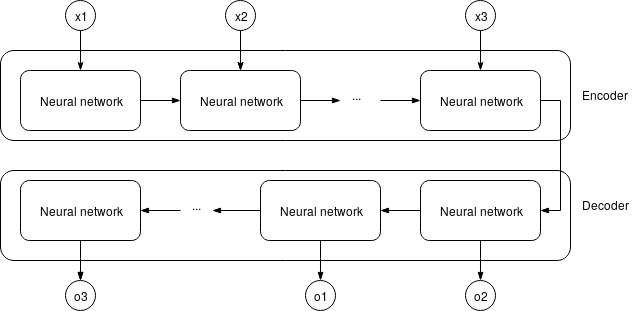
\includegraphics[width=\linewidth]{BasicEncoderDecoder.png}
    \caption{Generic Encoder-Decoder architecture, Neural network can be replaced by any form of Recurrent Neural Network}
    \label{fig:basic enc}
\end{figure}

\subsection{Bi-directional Long Short-Term Memory}
A known problem with the encoder-decoder network is their inability to 'remember' information in long input sequences \cite{attentionisallyouneed}. To solve this problem different methods have been proposed. One such method is the attention vector. An attention vector is an extra learned vector which points the decoder network towards important parts of the input sequence \cite{attentionisallyouneed}. Similarly, a coverage vector can be used to make sure that the decoder does not repeat itself often \cite{see2017get}. This repetition can be due to the aforementioned attention vector \cite{context}. Finally a BiLSTM model can also be used. 

To explain Bi-directional LSTMs, it is important to know how a normal LSTM works. An LSTM is a network that uses a time dependent hidden state ($c_t$) that keeps track of what the network has seen in the past. The network can choose to add knowledge into the hidden state and choose to forget knowledge. Below is shown that $h_{t-1}$ is an input. This assures that the future sequence is influenced by previous important features. Figure \ref{fig:LSTM} gives a graphical representation of the described LSTM, where small circles denote element wise operations and big circles are layers \cite{hochreiter1997lstm}.

\begin{figure}[H]
    \centering
    \includegraphics[width = \linewidth]{LSTM.png}
    \caption{Example LSTM, operation groups are overlaid for clarity.}
    \label{fig:LSTM}
\end{figure}

The value returned at timestep $t$ as the prediction is $h_t$. In order to overcome problems when a sequence starts and stops, special characters are used. These are often denoted as $<sos>$ and $<eos>$ for start and end of sequence respectively.

Figure \ref{fig:LSTM} shows that the output on the right feeds back into the cell of the left. Most publications shown this by repeating the same module. The weights associated with the LSTM are saved only once however \cite{hochreiter1997lstm}.

A biLSTM is an LSTM that is fed the input sequence from both directions. The double feeding of input is done because the LSTM long term memory is not as good as on would expect\cite{BiLSTM}. This technique makes it less likely to 'forget' information, as the information is fed from both sides of the input. The maximum distance the information can go is then halved \cite{BiLSTM}. Figure \ref{fig:BiLSTM} shows a graphical representation of how the BiLSTM explained.

\begin{figure}[H]
    \centering
    \includegraphics[width=0.8\linewidth]{BiLSTM.png}
    \caption{A generic BiLSTM that can be used for sequence2sequence predictions}
    \label{fig:BiLSTM}
\end{figure}{}

\section{Model design}
\label{design}
To automatically generate comments, a sequence to sequence model will be used. This has been shown to work effectively for NMT\cite{nguyen-le-etal-2017-improving}, code summarization \cite{alon2018code2seq} and comment generation \cite{hu2018deep} \cite{Hu2019}. The general architecture of the network will be discussed in this section; starting with an analysis of the dataset, then the processing of ASTs, followed by the encoding and decoding of input code.



\subsection{Dataset}
\label{dataset}
To compare the capabilities of the network with the current state of the art, the network is trained on the same dataset used by Hu et al in their deepcom network \cite{hu2018deep}. The dataset contains 588,108 code-comment pairs that can be used for training and evaluating, to keep it a fair test the same data split as in \cite{hu2018deep} will be used which is 80\% train, 10\% test and 10\% validation. See table \ref{tab:dataset-statistics} for the particulars.

\begin{table}[H]
    \centering
    \resizebox{\linewidth}{!}{
    \begin{tabular}{c c c c c}
    \# Methods   &  \# All tokens & \# All identifiers & \#Unique tokens & \#Unique identifiers\\
    \toprule
    588,108 & 44,378,497 & 13,779,297 & 794,711 & 794,621
    \end{tabular}}
    \caption{Statistics for codesnipets in DeepComm dataset}
    \label{tab:dataset-statistics}
\end{table}{}

The data set is generated from 9,714 Java projects that have been scraped from Github \cite{hu2018deep}.

Looking at the distribution of the comments (figure \ref{fig:fulldistr} we can see that it is extremely heavily biased towards short comments, however there are some comments that are more than 1500 words long. In order to get a better idea of how the data looks we also plot the distribution of only the comments less than 40 words in length in Figure \ref{fig:zoomeddistr}.

\begin{figure}[H]
    \centering
    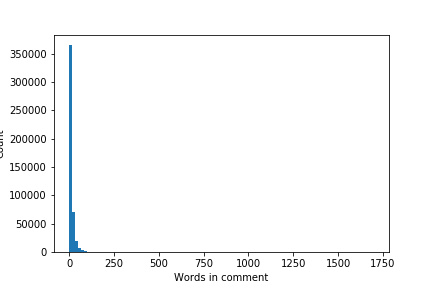
\includegraphics[width =0.9 \linewidth]{distr.png}
    \caption{Full distribution of comment lengths.}
    \label{fig:fulldistr}
\end{figure}{}

\begin{figure}[H]
    \centering
    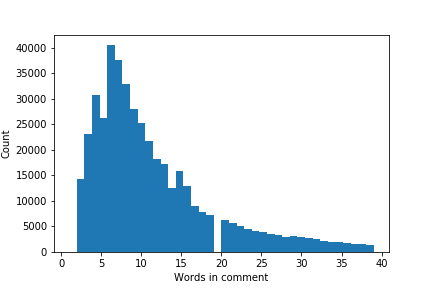
\includegraphics[width = 0.9 \linewidth]{zoomedInLength.png}
    \caption{Distribution of comment lengths below 40 words in length}
    \label{fig:zoomeddistr}
\end{figure}{}


After analysing the distribution we address the Out of Vocabulary problem (OOV). As mentioned before the OOV problem is the inability of an LSTM to predict words it has never seen before. This is because in code variable names are made up and  concatenation of different words in camel case or snake case do not matter.

Code summarization solves this by ignoring variable names. If you want to know whether you are dealing with a sorting algorithm, it doesn't matter what the variables are called. 
In Comment generation, the name of important variables can often be found in the comment. To make comments more natural the choice was made to replace the variables that appear in both the method and the comment by $"VARi"$ where $i \in \mathbb{Z}$ and $i$ is the index of the variable. The original variables are saved to a dictionary for every method. After comment prediction using the placeholder variables, these can be swapped out for the corresponding variables in the dictionary.


\subsection{AST}
\label{AST}
Luckily, working with code does have some advantages. Compared to more traditional natural language tasks, code contains a clear semantic relationship between the different lines of the code. This relationship can be used when creating an AST which is a graphical representation of the code, each node is a statement and the connections are the relations between the nodes. Figure \ref{fig:exampleAST} shows an example AST that is generated from function \ref{code:examplefunction}, as can be see from the leaves, the names of the variables have been replaced by VAR0 and VAR1, after the comment is generated they can be re-substituted for the correct names.

\begin{figure}[H]
    \centering
    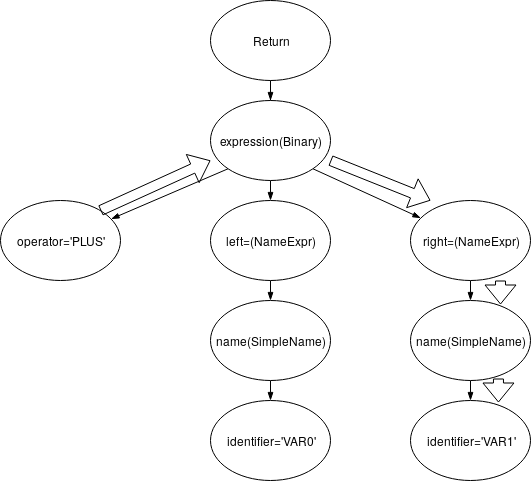
\includegraphics[width = 0.8\linewidth]{Embedding.png}
    \caption{Example AST of Function \ref{code:examplefunction}, the example path has been superimposed with thick arrows.}
    \label{fig:exampleAST}
\end{figure}

\lstinputlisting[language=Java, caption=Java example, frame=tb, backgroundcolor = \color{light-gray}]{example.java}
\label{code:examplefunction}


After the AST generation, this AST is encoded as suggested in \cite{alon2018code2seq} by randomly choosing up to $k$ leaf pairs that will represent a path. 

An example given the AST in Figure \ref{fig:exampleAST}, a valid pair would be $\{"Operator = 'PLUS'", "identifier=VAR1"\}$. The path belonging to this pair is 
\begin{multline}
\{"Operator 'PLUS'" \rightarrow "expression (BinaryExpr)" \\
\rightarrow "right(NameExpr)" \rightarrow "name(SimpleName)" \\
\rightarrow "identifier='VAR1'"\}
\end{multline}
The arrows in Figure \ref{fig:exampleAST} show this path. In general, each code snippet has a set of paths $\mathbb{V} = \{\{v_1,V_2,...,v_l\}, \{v^2_1, v^2_2,...,v^2_l\},\{v^k_1,v^k_2,...,v^k_l\}\}$ that is randomly sampled before each training session. This enables the model to learn that small differences in code like the use of a while loop or a for loop are not as important. It is re-sampled every time before training in order to ensure that the training is fair\cite{alon2018code2seq}.


\subsection{Encoding}
\label{Encoding}
Our model is trying to solve a sequence to sequence problem. The architecture used is a encoder decoder structure. To decode to a sequence, first the input sequence needs to be encoded. 
In this model a Bi-LSTM is being used for both encoding and decoding. Whilst encoding it takes as input sequence a set of paths through the AST \cite{alon2018code2seq}. Terminal nodes are split into subtokens which sum up to be tokens, using a learned embedding in the network. 

Once this is done there are 3 main elements. From the start node of the path and the end node of the path there are 2 embedded tokens. The path through the AST is also encoded into an embedding. These are combined by concatenating all 3 parts and feeding them in to a fully connected layer which calculates the output of the encoder \cite{alon2018code2seq}. A graphical representation of this can be seen in \ref{fig:encoder}.

\begin{figure}[H]
    \centering
    \includegraphics[width =\linewidth]{Encoder(1).png}
    \caption{Graphic representation of Encoder, $Encode(x) = \sum_{s\in x} E^{\text{subtokens}}_s$}
    \label{fig:encoder}
\end{figure}{}

As can be seen from the described architecture, there is a hard limit to the length of the paths in an AST, which will indirectly limit the length of the functions that can be processed. 

\subsection{Decoding}
\label{decoding}
After passing through the encoders fully connected layer, the embeddings areare passed to another BiLSTM. This BiLSTM transforms the hidden state it receives into a highest probability embedding. This encoded embedding is then decoded to the corresponding human readable word.

To assist the BiLSTM generating a sequence, an attention mechanism is added over the output of the encoder. The attention vector helps the decoder to 'Attend' to important information. This vector is an extra weight vector applied to the output\cite{attentionisallyouneed}.

\section{Experimental setup}
\label{setup}

In this section we show the setup of our project. We describe the data used and the network configuration for each of the 2 experiments we conducted. Then the evaluation metric utilized for our experiments  and the reason why this is the proper quality measure for our case.

We run the experiments in two folds. For the first one (\textit{Method-1}), we used the architecture of the Code2Seq paper to train a model with the dataset used in the DeepCom paper, while for the second one (\textit{Method-2}) we used the same architecture enhanced with the inclusion of changed ASTs. This task challenging by the process of generating comments instead of the predicting function names is difficult. This difficulty arises from the fact that comments are usually longer than function names. Also, we are generating natural language instead of a sequence of descriptive words. The results of both methods are then compared with the results of the DeepCom\cite{hu2018deep} as the baseline. For each of these 2 experiments, we calculated the BLEU score as a measure for the quality of the obtained results.


\subsection{Experiments}

For our first experiment (\textit{Method-1}), we modified the Java AST extractor used in Code2Seq. Instead of using the name of the examined function of the Java snippet, we used the comment for this function as target for our model to generate a comment for the snippet instead of a name. Regarding the model hyperparameters, we slightly modified the ones proposed by the Code2Seq paper for the Code Captioning task. We optimized the cross-entropy loss with a Nesterov momentum of 0.95. The learning rate was 0.01 and decayed by 0.05 every epoch. We applied dropout of 0.3 and a recurrent dropout of 0.5 on the LSTM encoding the AST paths. The embeddings size was 128, the same as the batch size. The encoder LSTM had 256 units while the decoder one had 640 units. The reason for the large amount of units in the decoder LSTM is that the target of our network (comments) is long enough. Finally, 200 paths were chosen from each of the extracted ASTs. We trained the model for 100 epochs, while we applied early stopping if no improvement was noticed for 10 epochs. The  trainable parameters for this model are 38469376.

When it comes to our second experiment (\textit{Method-2}), we repeated the first experiment with modified ASTs. Instead of using each variable (leaf of the AST) with a generic name (e.g Var1) and its type only, we also added the actual name of the variable \cite{ZHOU2019328}. The  trainable parameters for this model were 34230144.

\subsection{Evaluation}
The main evaluation metrics for the comments generated by our models was the Bilingual evaluation understudy (BLEU-4) \cite{Papineni:2002:BMA:1073083.1073135}. BLEU measures the quality of  a translation (in our case from source code to comments) with a corpora of possible translations. It is widely-used to measure the accuracy of Neural Machine Translation (NMT) \cite{klein2017opennmt}. BLEU measures how close the output of the machine is to the one of a human expert. The closer they are, the higher the BLEU score will be \cite{ward2002corpus}. The BLEU score ranges between 0 and 1, with 1 being perfect natural language. BLEU has shown a high correlation with human quality judgement \cite{callison2006re} and is one of the most popular metrics to measure the the quality of machine translated text.

The BLEU score for each of the examined snippets is calculated and their average value is computed as our final evaluation result. BLEU calculates the n-gram similarity and uses this to come up with a score according to the equation:
$$BLEU = BP \cdot exp \left (\sum^{N}_{n=1}w_n\log p_n   \right )$$
Where in our case $BP = 1$ as the reference corpus is only 1 comment per code snippet. $w_n$ is a weight vector that sums to 1, $p_n$ is the modified n-gram precision, and N is the max length of n-grams being used in the comparison\cite{Papineni:2002:BMA:1073083.1073135}, which in our case is N=4.

We also measured precision, recall, and F1 score as  used in \cite{allamanis2016convolutional} and \cite{alon2019code2vec} over all the sub-tokens of the target sequence, case insensitive.

\section{Results}\label{results}
The results of both the methods - Method-1, which uses the code2seq based natural language prediction and Method-2, which used the Method-1 along with modified ASTs (solving out of vocabulary problem). The results will be discussed in terms of the BLEU-4 score, precision, recall and the actual comments generated during testing. For comparing the predicted comments, we used the same java codes as presented in the DeepCom paper \cite{hu2018deep}.

%%%%%%%%%%%%%%%%%%%%%%%%%%

\begin{table}[H]
\centering
\begin{tabular}{cc}
\hline
Approaches & BLEU-4 score \\ \hline
DeepCom & 38.17 \\
Method-1 & 6.08 \\
Method-2 & 10.02 \\ \hline
\end{tabular}
\caption{Evaluation results on Java Methods}
\label{tab:bleu-table}
\end{table}
%%%%%%%%%%%%%%%%%%%%%%%%%%
\begin{table}[H]
\centering
\begin{tabular}{cccc}
\hline
Approaches & Precision & Recall & F1 \\ \hline
Method-1 & 36.26 & 21.56 & 27.04 \\
Method-2 & 46.94 & 27.44 & 34.63 \\ \hline
\end{tabular}
\caption{Performance on Java code}
\label{tab:prec_recall}
\end{table}
%%%%%%%%%%%%%%%%%%%%%%%%%%

Table \ref{tab:bleu-table}, presents the BLEU-4 scores achieved by the baseline and our Methods-1,2. Table \ref{tab:prec_recall} presents the precision, recall and f1 scores of our methods. Finally, table \ref{tab:results} presents the comments generated by our models with respect to the java codes and results presented in DeepCom \cite{hu2018deep}.

Table \ref{tab:bleu-table} shows that both our methods fails to improve over the baseline - Deepcom. The poor performance can be due to the imbalanced distribution of target comment lengths in the dataset (as seen in Fig-\ref{fig:fulldistr}, \ref{fig:zoomeddistr}) and to the fact that the code2seq based learning architecture (adopted by the methods) was built to predict function names and not natural language. This tends to predict comparatively shorter comments. The evaluation metric (BLEU-4), is 4-gram based comparison technique, and severely punishes our shorter comments. It is also important to note that the Method-2 out performs the Method-1 confirming the effectiveness of solving the problem of \textit{Out of Vocabulary} in ASTs. Similar results are seen in the Table-\ref{tab:prec_recall} too, where the Method-2 out performs the Method-1. Hence, an important takeaway is that ASTs generally hold the problem of \textit{Out of Vocabulary} affecting the training process, hence, a suitable AST generation technique (e.g. \cite{ZHOU2019328} - the one used by Method-2) should be used to avoid such problem.

\end{multicols*}
% \lstset{style=mystyle1}
\newgeometry{left=2cm,right=0.25cm,bottom=0.25cm,top=0.25cm}
\begin{landscape}
% \vspace{1 cm}
    \begin{table}[H]
    % \rowcolors{1}{}{lightgray}
    \resizebox{29.cm}{!}{
    \begin{tabular}{c l l l l l}
    % \hline
    Case ID & \multicolumn{1}{c}{\itshape Java Method} & 
    \multicolumn{1}{l}{\begin{tabular}[l]{@{}l@{}}\itshape Human-written \\ \itshape comments\end{tabular}}
    & \multicolumn{1}{l}{\begin{tabular}[l]{@{}l@{}}\itshape DeepCom\\ \itshape comments\end{tabular}} & \multicolumn{1}{@{}l@{}}{\itshape Method - 1} & \multicolumn{1}{@{}l@{}}{\itshape Method - 2} \\ \toprule
    1 & 
    % \begin{tabular}[c]{@{}l@{}}
    \lstinputlisting{source-code/1.java}
    % \end{tabular} 
    & Convert Bitmap to byte array & Convert Bitmap to byte array & Convert a bitmap to a byte. & Serialize an array of png into. \\ \hline
    2 & 
    % \begin{tabular}[c]{@{}l@{}}private static void addDefaultProfile(SpringApplication app,                                                            \\                           SimpleCommandLinePropertySource source)\{\\   if(!source.containsProperty("spring.profiles.active") \\   \&\&!System.getenv().containsKey("ACTIVE"))\{\\      app.setAdditionalProfiles(Constants.DEVELOPMENT);\\ \} \}\end{tabular} 
    \lstinputlisting{source-code/2.java}
    & \begin{tabular}[c]{@{}l@{}}If no profile has been configured,\\ set by default the "dev" profile.\end{tabular} & \begin{tabular}[c]{@{}l@{}}If no profile has been configured,\\  set by default the "dev" profile.\end{tabular} & Checks if the var is active. & If not active, set additional profiles. \\ \hline
    3 & 
    % \begin{tabular}[c]{@{}l@{}}
    % public FactoryConfigurationError(Exception e)\{\\          super(e.toString());\\         this.exception=e;\\ \}
    % \end{tabular}
    \lstinputlisting{source-code/4.java}
    & \begin{tabular}[c]{@{}l@{}}Create a new FactoryConfigurationError\\  with a given Exception base cause of the error.\end{tabular} & \begin{tabular}[c]{@{}l@{}}Create a new <UNK>\\ with a given Exception base cause of the error.\end{tabular} & -NA- & -NA- \\ \hline
    4 & 
    \lstinputlisting{source-code/3.java}

    % \begin{tabular}[c]{@{}l@{}}
    % protected void createItemsLayout()\{ \\         if (mItemsLayout == null)\{\\                 mItemsLayout=new LinearLayout(getContext()); \\                 mItemsLayout.setOrientation(LinearLayout.VERTICAL);\\ \} \}\end{tabular} 
    & Creates item layout if necessary & Creates item layouts if any parameters & Creates the layouts layout. & Creates item layouts if necessary.  \\ \hline
    5 & 
    \lstinputlisting{source-code/5.java}

    % \begin{tabular}[c]{@{}l@{}}public static void sort(Comparable{[}{]} a)\{ \\         int n=a.length;\\         for (int i=1; i \textless n; i++)\{ \\                 Comparable v=a{[}i{]};\\                 int lo=0, hi=i;\\                 while (lo \textless hi) \{ ... \} \\                 ...\\         \}\\         assert isSorted(a);\\ \}\end{tabular} 
    & \begin{tabular}[c]{@{}l@{}}Rearranges the array in ascending order,\\ using the natural order.\end{tabular} & \begin{tabular}[c]{@{}l@{}}Sorts the array in ascending order,\\  using the natural order.\end{tabular} & Sorts the var with the given. & Sort a set of entries based. \\ \hline
    6 & 
    \lstinputlisting{source-code/6.java}
    % \begin{tabular}[c]{@{}l@{}}public boolean isEmpty()\{\\         return root == null;\\ \}\end{tabular} 
    & Is this symbol table empty? & Returns true if the symbol is empty. & Returns true if the tree is. & Returns true if the symbol empty. \\ \hline
    7 & 
    % \begin{tabular}[c]{@{}l@{}}public boolean contains(int key)\{\\         return rank(key) != -1;\\ \}\end{tabular} 
    \lstinputlisting{source-code/7.java}
    & Is the key in this set of integers? & \begin{tabular}[c]{@{}l@{}}Checks whether \\ the given object is contained within the given set.\end{tabular} & Returns true if the key is. & Returns true if this symbol contains. \\ \hline
    8 & 
    % \begin{tabular}[c]{@{}l@{}}public void tag(String inputFileName,String outputFileName,\\                                OutputFormat outputFormat)\{\\          List sentences=jsc.textFile(inputFileName).collect(); \\         tag(sentences,outputFileName,outputFormat);\\ \}\end{tabular} 
    \lstinputlisting{source-code/8.java}
    & \begin{tabular}[c]{@{}l@{}}Tags a text file,\\ each sentence in a line and writes the result to an output file\\ with a desired output format.\end{tabular} & Replaces the message with a given tag. & This method is called when executing. & This method is used to process. \\ \hline
    9 & 
    % \begin{tabular}[c]{@{}l@{}}public void unlisten(String pattern)\{\\    UtilListener listener=listeners.get(pattern); \\    if(listener!=null)\{\\        listener.destroy();\\        listeners.remove(pattern); \\    \}else\{\\       client.onError(Topic.RECORD,Event.NOT\_LISTENING,pattern);\\ \} \}\end{tabular} 
    \lstinputlisting{source-code/9.java}
    & \begin{tabular}[c]{@{}l@{}}Removes a listener \\ that was previously registered with listenFor - Subscriptions.\end{tabular} & \begin{tabular}[c]{@{}l@{}} It can be called when the product \\ only or refresh has ended.\end{tabular} & Removes a var from the topic. & Removes the message from the listener. \\ 
    % \hline
    \end{tabular}}
    \caption{Comment Generation Results}
    \label{tab:results}
    \end{table}
\end{landscape}
\restoregeometry
%%%%%%%%%%%%%%%%%%%%%%%%%%
\begin{multicols*}{2}

Post the preliminary analysis of quantitative results as above, we wanted to analyse the comments generated by our models in a qualitative manner. Such a qualitative analysis is critical, specially for the task at hand (Comment generation), as a qualitative analysis of the comments may explain whether the model has learnt the \textit{syntactic and semantic meaning} from the code to generate comments. For this task, we used the same java codes as used by our baseline paper \cite{hu2018deep}. This will help us derive unbiased insights in to the comment generation capability of out models (Method-1,2). Table-\ref{tab:results}, presents these results. From the Table, we see that while compared to the \textit{Human-written} and \textit{DeepCom} comments, the comments of \textit{Method-1,2} are quite shorter, nearly half of its size. As discussed earlier, this could be the reason for the poor BLEU score. Nevertheless, by looking deeper, we see that almost all the comments generated by Method-1,2 has infact learnt the true syntactic and semantic meaning of the java code. In all cases the comments generated by our methods captures the crux of the java code, verifiable using the  \textit{Human-written} and \textit{DeepCom} comments. For Example, In Case-1 and 5, we see that our best model (\textit{Method-2}), understands the main concept of the code, i.e. the concept of \textit{image processing} and \textit{sorting} respectively. But it fails to finish the comment and leaves it abruptly, due to the method's inability to predict longer natural language comments. Nevertheless, In some cases like Case-2, 3, 6, 7, it performs perfectly and very similar to the human written comment, sometimes better than the baseline DeepCom itself (i.e in Case 4). Hence, The main conclusion we can draw from these results is that, our best model - \textit{Method-2}, is capable of understanding the \textit{syntactic and semantic meaning} of java codes to generate comments automatically, but suffers from the incapability to generate longer and complete comments.



\section{Discussion}
\label{discussion}

In the first experiment we conducted we were not able to build a model that can generate proper comments. The generated comments were much shorter than the original ones while they were less descriptive. However, after applying the preprocessing step, in which we included the variable name in the ASTs, we observed a satisfactory increase in the BLEU-4 score achieved. This suggests an increased quality of generated comments. The using of more specifically linked variables in both comment and code resulted in making the comments more accurate. 

By visually inspecting the comments generated from our second experiment, it can observe that the generated comments are quite close to the ones written by human. Comments generated by our model tended to be short, which led to a low BLEU-4 score. This issue is caused by the fact that Code2Seq model was built for another purpose, which differs significantly from the comment generation process. The Code2Seq model was built for generating function names which are shorter and not so structured as a comment. Better results may have been achieved if we had the time and the computational resources to experiment with some of the model hyperparameters (e.g. increasing the decoder size). Despite the improvement achieved by the inclusion of the variable name in the ASTs, we believe that a lot of work need to be done upon building a model which can work properly in a real case scenario.

Looking back at the dataset that was used, it may have been beneficial to filter out some of the methods with shorter comments. This because the distribution of comment length is heavily biased towards short comments. It may also have been helpful to filter out methods in general with comments that have a length of less than about 4 words, assuming that for a clear and descriptive comments slightly longer comments are preferred. Re-balancing the dataset so each length has an equal representation would also have been a good idea. This would either require a special form of data augmentation, over-sampling, or under-sampling.

Keeping the contribution of this paper in mind, any future works should work towards improving the models capability to generate longer and complete comments. While this paper concentrated more on the AST generation and encoder modules of the model, future works should deploy a more suitable decoder module for the target natural language comments.


\section{Conclusion}
\label{conclusion}
Automatic comment generation for Java code can be very beneficial. Both for readability of old code, but also better comment suggestions as a programmer aid. With DeepCom as the baseline, this paper focused on replicating the code2seq model with added capabilities such as, predicting natural language (Method-1) and modified ASTs (Method-2). From our results we see that both our methods do not perform as good as the baseline in terms of the BLEU-4 scores. However, Method-2 was much better then our first method. With Method-2 as our best method, an important takeaway is that ASTs generally hold the problem of \textit{Out of Vocabulary} affecting the training process and a suitable AST generation technique (e.g. \cite{ZHOU2019328} - the one used by Method-2) should be used to avoid such problem. Nevertheless, looking at the comments generated by our best performing model (Method-2), we see that Method-2 is capable of understanding the \textit{syntactic and semantic meaning} of java codes to generate comments automatically, but suffers from the incapability to generate longer and complete comments.

% This research focused on a model that has been proven to work well, and is one of the best performing comment generators at the moment. Our decision to replace a part of this model with the new state of the art code2seq seemed like a good idea, given the much improved results that were found by the author of code2seq. Our results however paint a different picture, but we do not believe that this is because of the model not working, but simply time constrained that left us with too little training and hyper parameter tuning time. Our results speak for themselves. They are much worse than the model we tried to improve. There is a silver lining though.  We believe that we are on the right track with our method-2 model, and given time be able to beat DeepCom.

We would like to thank our teachers Georgios Gousios and Maurício Aniche for their help and suggestions. We would also like to thank all our fellow classmates from the IN4334 class of 2019 for their interest in our presentations, though and interested questions, and their own presentations with good discussions in return.


\section{Reflection}
\label{reflection}
In retrospect we find that this project was a partial success. From the start we found that it was a very manageable amount of work with a clearly defined goal.

The research phase went well and we quickly had a clear goal of what we wanted to achieve and how we wanted to get there. We are happy how this worked out and feel that everyone in the group has a better understanding of how NMT works as well as a better understanding of the mechanisms used such as the BiLSTM, ASTs and attention mechanisms. 

The area that we struggled the most with was the implementation. As we wanted to build upon other research we needed to adapt code that was released along with the papers. This sounded like a good idea at the start. However, after a a few weeks we were having problems with understanding the code written by the original researchers and we spent many hours going through the JavaExtractor code, which ironically was hard to understand as none of it was documented/had comments. 

Once we did finally manage to change the JavaExtractor to replace the variables with VARi it was unfortunately rather late in the project from which our training time suffered as we could not do all the runs that we had wanted to. Looking back, it would have been better to start the changing of the JavaExtractor earlier, as we already knew we wanted to do this at the start of the research phase, but chose to focus on research first and only afterwards start with editing/implementing.

Nevertheless, we were able to train two different models (Method- 1,2) and contribute to the automatic generation comments to java codes. An important takeaway from the results is that ASTs generally hold the problem of variable names affecting the training process, hence, a suitable AST generation (e.g. \cite{ZHOU2019328} - the one used by Method-2) to avoid such problem. Hence, the main conclusion that we can draw regarding our best model - \textit{Method-2}, is that, our model is capable of understanding the \textit{syntactic and semantic meaning} of java codes regarding the automatic comment generation, but suffers from the incapability to generate longer comments and complete. 

% \newpage
\bibliographystyle{unsrt}
\bibliography{reference}
\end{multicols*}


\newpage
% \section{Appendix}\label{s:app}


\end{document}
